        \documentclass[11pt,oneside,a4paper]{scrartcl}
\renewcommand{\familydefault}{\sfdefault}
\usepackage{amsmath}
\usepackage{helvet}
\usepackage[utf8x]{inputenc}
\usepackage[english]{babel}
\usepackage{fancyhdr}
\usepackage{graphicx,caption}
\usepackage{subfig,amsmath}
\usepackage{setspace}
\usepackage{longtable}
\usepackage{wasysym}
\usepackage{geometry}
\usepackage{gensymb}
\usepackage{color}
\usepackage{colortbl}
\geometry{a4paper,left=2cm,top=1cm, top=1.5cm, bottom=3.5cm}
\makeatletter
\renewcommand\paragraph{\@startsection{paragraph}{4}{\z@}%
  {-3.25ex\@plus -1ex \@minus -.2ex}%
  {1.5ex \@plus .2ex}%
  {\raggedsection\normalfont\sectfont\size@paragraph}%
}
\makeatother
%\renewcommand\thesection{\arabic{section}}

\begin{document}

\vspace*{1cm}
\pagestyle{fancy}
\fancyhf{}
%Kopfzeile rechts bzw. au�en
\fancyhead[RO]{Florian Kraemer}
%Kopfzeile links bzw. innen
\fancyhead[LO]{\today}
%Linie oben
\renewcommand{\headrulewidth}{0.5pt}
%Linie unten
\renewcommand{\footrulewidth}{0.5pt}
\addtolength{\headheight}{30pt}



\vspace*{2cm}
\begin{center}
\vspace*{0.5cm}
\textbf{\Huge Sensordata}
\vspace*{2cm}
\\ An android-application to read, store and display compressed sensordata\\
\end{center}

\vspace*{3cm}

\begin{center}
\textbf{\LARGE} Florian Kraemer \\
\end{center}

\newpage % Ende vom Text

\tableofcontents

\newpage

\setcounter{page}{1}
\pagestyle{fancy}
\fancyhf{}
%Kopfzeile rechts bzw. aussen
\fancyhead[RO]{Florian Kraemer}
%Kopfzeile links bzw. innen
\fancyhead[LO]{\textbf{\large Sensordata}}
%Linie oben
\renewcommand{\headrulewidth}{0.5pt}
%Fu�zeile rechts bzw. au�en
\fancyfoot[C]{\thepage}
%Linie unten
\renewcommand{\footrulewidth}{0.5pt}
%\addtolength{\headheight}{10pt}

\onehalfspacing
\setcounter{section}{0}

\section{Objective}
Smartphones offer a wide range of use. We want to use their fair processing power, storage capacity and attached sensors to allow easy handling of sensor networks. Thus the task is to develop an android application that is capable of receiving data from sensor nodes via the telecommunication network, processing, storing and displaying them in a significant way. Furthermore managing the metadata of each node on a phone will make it user-friendly to find nodes, alter positions in an existing sensor-network or install new nodes. Challenges are to keep the application as modular as possible, to allow changes to the supported sensor-network, like for example the number of sensors, the number of platforms or switching between compression algorithms. The smartphone is also not intended for storing the data forever. Possibly having smartphones in the field and their hardware capabilities requires to backup the data regularly. But connecting to a web-service would also allow for using for example a tablet just for displaying data. It is also important to make the application usable on different devices featuring different screen sizes and processing power or telecomunication features.

\subsection{The supported sensor-platform}
The current release of the application supports a platform with four sensors, each having two subsensors, one for moisture- and one for temperature measurements. An additional sensor is used to collect battery data. The data is then compressed with a Huffman-Code, a method developed by Rachel Cardell-Olivier, and transmitted in a SMS-message.


TODO insert footnote
\section{Architecture}
\subsection{Overview}
The application features several activities for the different types of user-interactions. \\
Then there is an underlying service, that handles the background data-processing. It reads, decompresses and stores the sensordata from the phone's SMS-inbox. It also handles which numbers are interpreted to be platforms and to which platform in the database they should correspond Besides this it also provides the connection between the activities and the database.

\subsection{Data model}
An existing data model  FOOTNOTE was reduced to fit the specifications of a smartphone application. This reduces the amount of choices the user has to make in order to operate and keeps the complexity to a certain level. It also makes the database as lightweight as possible. The measurement entity-type features no dedicated id, but instead the timestamp and subsensor id are used as a unique primary key.

\begin{center}
\begin{tabular}{|c|c|}
\hline \textbf{ Entity-type} &  \textbf{Attributes} \\ 
\hline platform & id,description,period,latitude,longitude,mobile number \\ 
\hline sensor & id,latitude offset, longitude offset, elevation offset, platform id \\ 
\hline subsensor & id, phenomena id, sensor id \\ 
\hline measurement & timestamp, measurement, subsensor id \\ 
\hline phenomena & id, description, unit, maximum, minimum \\ 
\hline 
\end{tabular} 
\end{center}


\section{Implemention}
\subsection{Activities}
The current release uses just five activities. This is possible due to recycling of two of them: Depending on the intent they are started with, the choose-a-platform-activity and the change-a-platform-activity react differently. This makes sense, since very similar actions like altering and inserting new metadata for a platform require the same layout and it prevents duplicate code.

\begin{center}
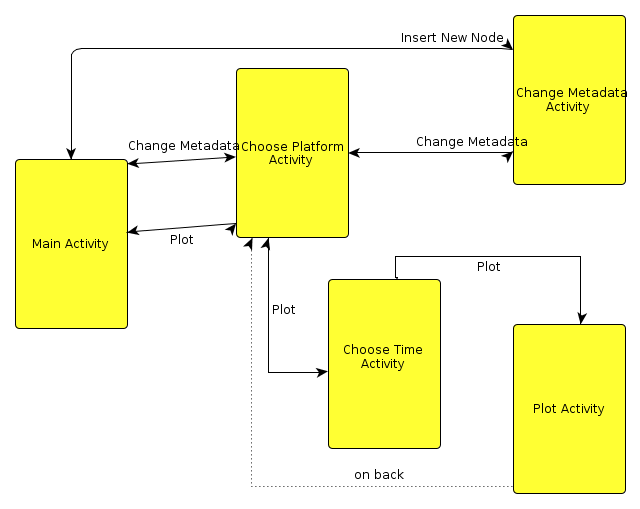
\includegraphics[scale=0.6]{picture/sensordata_activities.png}\\
\textit{Graph of activities}
\end{center}

\subsubsection{Main}

\subsubsection{Choose Platform}

\subsubsection{Change Platform}

\subsubsection{Choose Time}

\subsubsection{Plot data}
\subsection{Plotting}
To visualize the data the library androidplot is used. It offers a wide range of preferences, but a rather sparse API. The biggest challenge here is to find the limits for displaying as much data as possible while still making it wel-readable and handable for the user. Thus it might just be a well-sized extract from the chosen data.
Since the plots are implementing a touch functionality, the shown ranges are limitted with maximum and minimum values, so one can not get lost in the depth of the graph. 
To make the touch experience a bit smoother, a thread was implemented, that slows the scrolling and zooming exponentially down after the touch gesture, instead of stopping immediately.
To not allow the view to be scrolled on smaller screen sizes a custom scrollview was implemented, that allows to block scrolling the view while gestures are made on the plots.

\subsection{Thread safety}
The android platform comes with a mannerism, that necessitates special handling at times. The most important constraint is that changes to the views can only be done from the UI-thread. When using multithreading thus attention must be paid to this. The android API provides the AsyncTask, its onPostExecute is executed in the UI-thread and can therefore be used to meet this challenge.
In the current release CountdownLatches are used to prevent from problems upon binding to the underlying service. This process takes some time and when put for example in the OnStart-method of an activity, it is not reliably executed at the expected time.


\end{document}
